\chapter{Modélisation probabiliste}

L'objectif est ici de simuler explicitement l'effet des incertitudes au sein du code \textbf{CROCO}. Pour cela, les travaux de \oldcite{brankart_generic_2015} sur le modèle \textbf{NEMO} servent de base de développement. Dans ce chapitre, nous décrivons tout d’abord les processus stochastiques utilisés, avant de détailler leur implémentation dans le modèle en suivant la méthodologie de \oldcite{weiss_probabilistic_2025}.

\section{Processus stochastiques}

Les perturbations stochastiques ont été implémentées explicitement dans le modèle \textbf{CROCO} via un développement dédié. Cette implémentation repose sur l'utilisation du module \textbf{STOGEN}, conçu pour générer des champs de variables aléatoires spatialement et temporellement corrélés, et les injecter dans le modèle à chaque pas de temps.

Le module \textbf{STOGEN} \cite{brankart_generic_2015} permet de produire des champs stochastiques gaussiens autorégressifs selon les propriétés statistiques définies~: moyenne, écart-type, et temps de corrélation.

Une attention particulière a été portée à la neutralité des perturbations vis-à-vis de la moyenne. En effet, pour éviter l’introduction d’un biais systématique dans les simulations, les champs sont centrés autour de $1$ avant injection, comme illustré en \autoref{fig:sto dist}.
\begin{figure}[h]
\centering
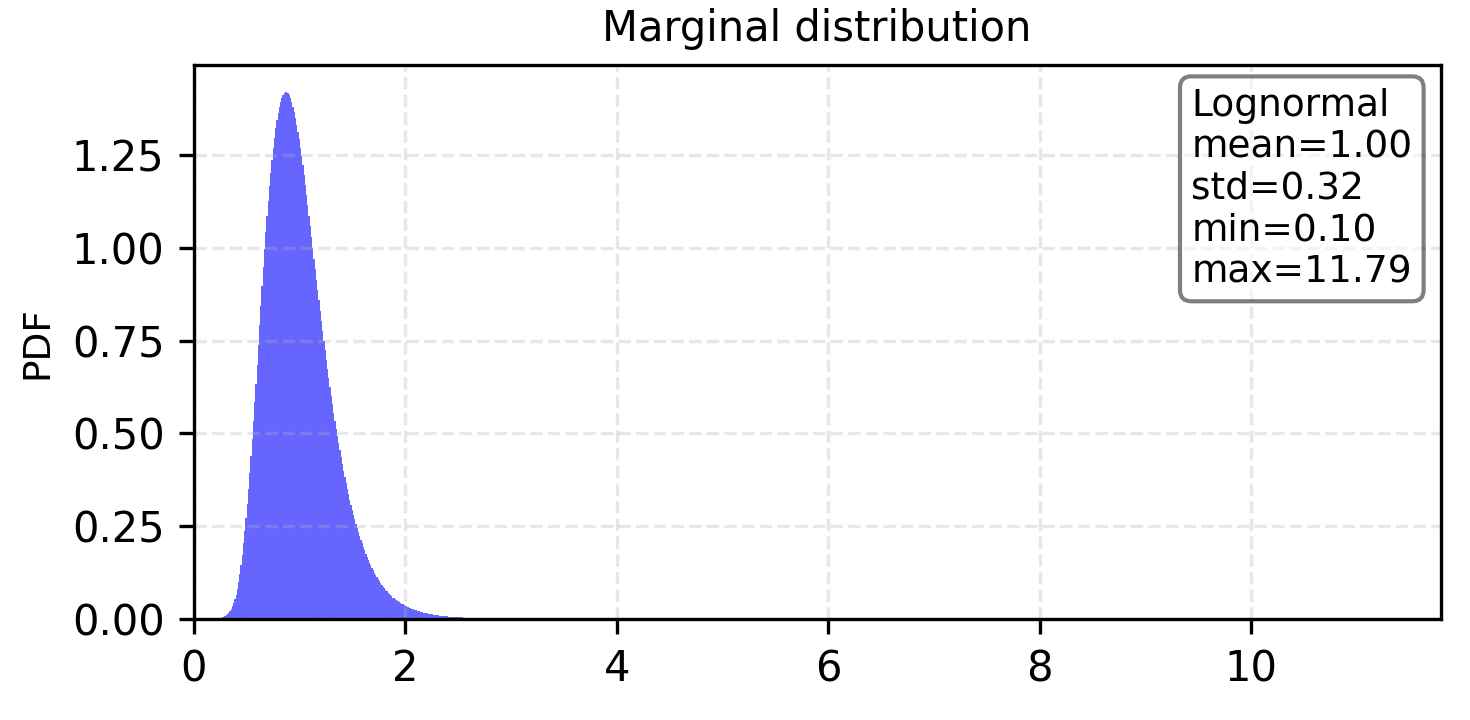
\includegraphics[width=0.7\textwidth]{Figures/sto_dist_lap_dist}
\caption{Distribution marginale du processus stochastique pour un membre}
\label{fig:sto dist}
\end{figure}

Les processus stochastiques élémentaires utilisés ici sont des processus autorégressifs gaussiens $\xi^{(i)}$, générés en chaque point de grille $i = 1, \ldots, m$ selon l’\autoref{eq:autoregressive process} :
\begin{equation}
	\label{eq:autoregressive process}
	\xi_{k+1}^{(i)} = a^{(i)} \xi_{k}^{(i)} + b^{(i)} w^{(i)} + c^{(i)}
\end{equation}
où les coefficients $a^{(i)}$, $b^{(i)}$ et $c^{(i)}$ définissent la moyenne souhaitée $\left(\mu^{(i)}\right)$, l’écart-type $\left(\sigma^{(i)}\right)$ et le temps de corrélation $\left(\tau^{(i)}\right)$ de $\xi^{(i)}$.

Une corrélation spatiale est ensuite introduite à l’aide d’un filtre laplacien horizontal appliqué à plusieurs reprises. Cette opération permet de générer des structures corrélées dans l’espace, dont l’échelle spatiale est compatible avec celle de l'incertitude que l'on souhaite décrire, comme illustré en \autoref{fig:sto spatial}.

Après une centaine d’itérations du filtre laplacien, on obtient une distribution présentant une corrélation spatiale significative, avec des structures de taille comparable aux tourbillons méso-échelles.
\begin{figure}[h]
\centering
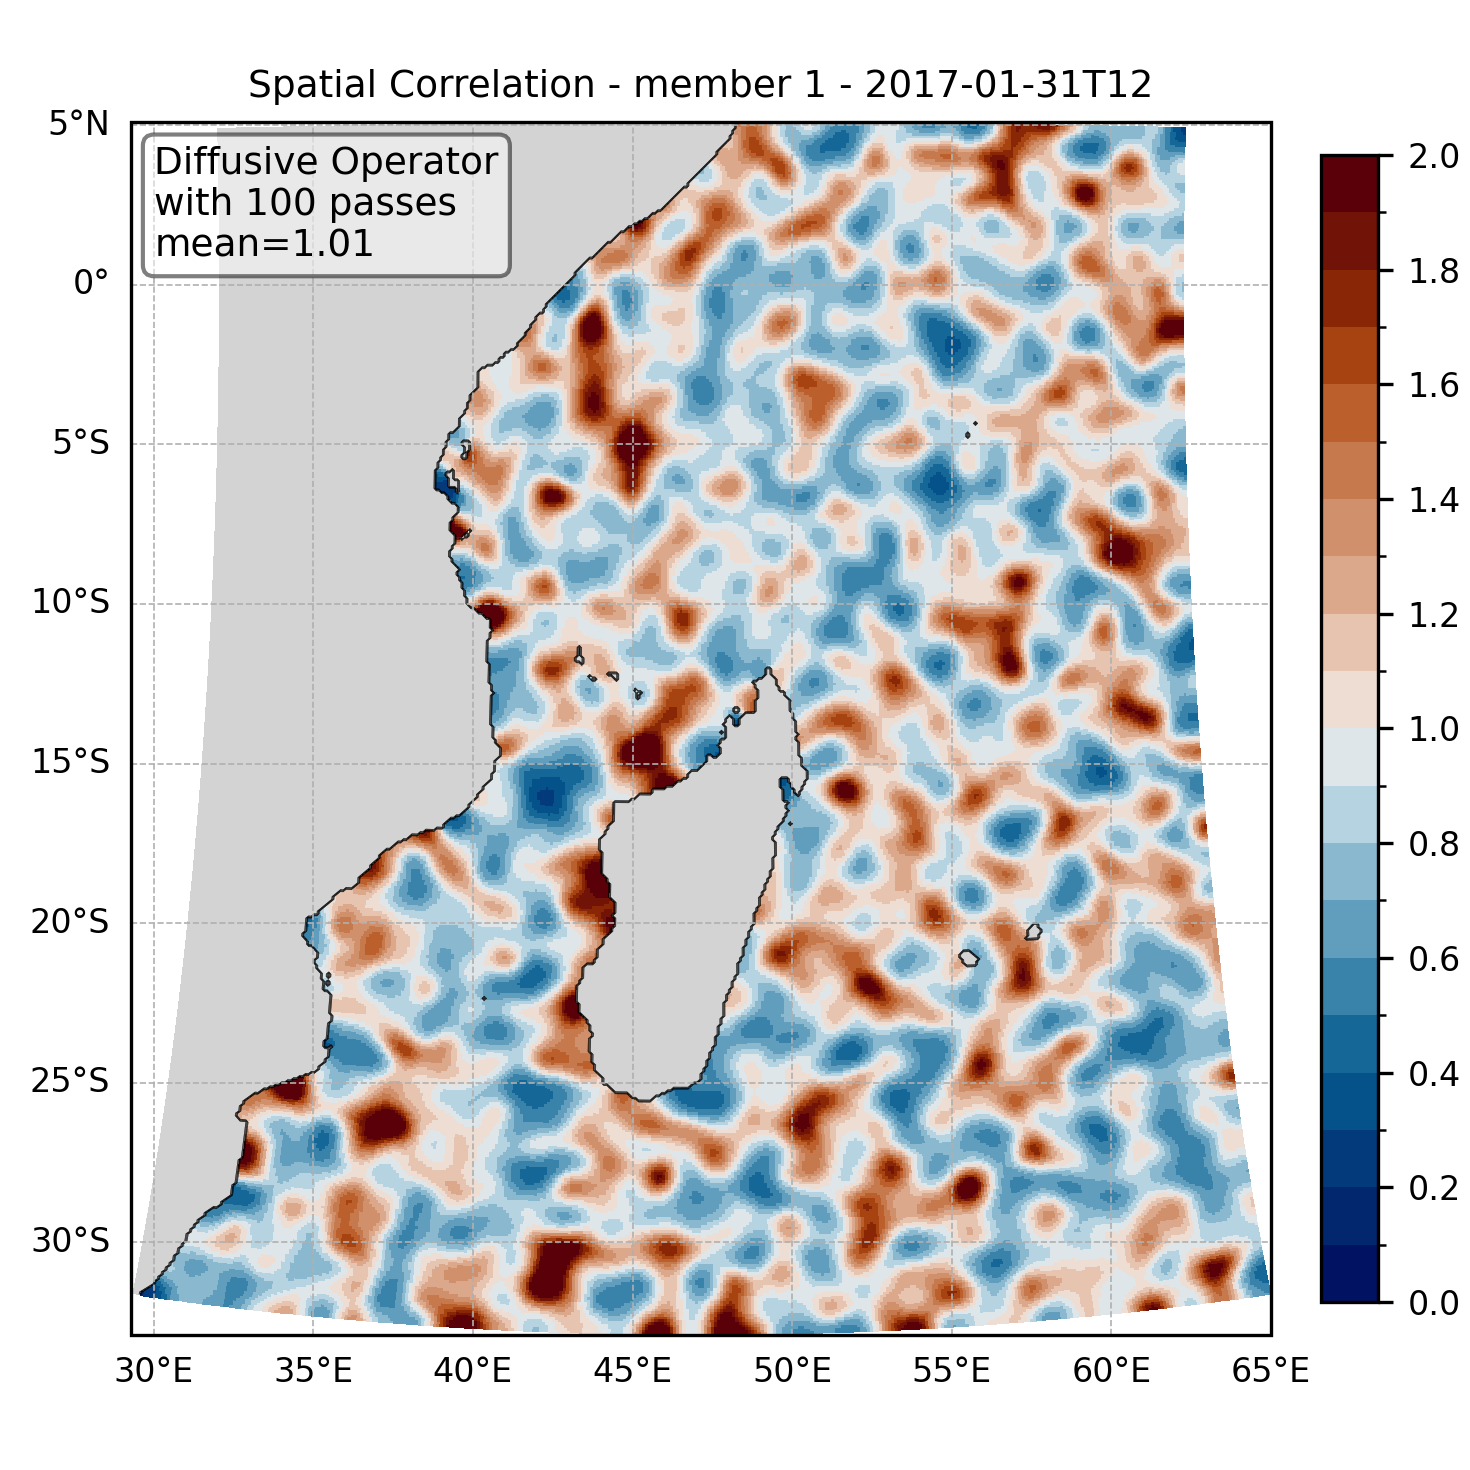
\includegraphics[width=0.7\textwidth]{Figures/sto_dist_lap_spatial}
\caption{Distribution spatiale du processus stochastique pour un membre}
\label{fig:sto spatial}
\end{figure}

\section{Perturbation des équations}
\subsubsection{Ensemble étudiant le mélange vertical}

Ce premier ensemble nous permet d'étudier l'impact d'une perturbation de la paramétrisation du mélange vertical définie en \autoref{eq:GLS}

La perturbation du schéma de paramétrisation verticale de l’énergie cinétique turbulente (TKE) a nécessité un travail plus approfondi. Une revue bibliographique a été menée pour identifier des travaux antérieurs portant sur ce type de perturbation. Les travaux de \oldcite{juricke_stochastic_2017} ont étudié l’impact de perturbations stochastiques appliquées à différentes paramétrisations du mélange vertical dans un modèle océanique global à résolution $1^{\circ}$. Leur modèle utilisait une équation prognostique de la \textbf{TKE} similaire à celle donnée en \autoref{eq:tke prog}, ce qui rend leur démarche transposable au modèle \textbf{$k$–$\varepsilon$} utilisé ici.

Ainsi, les champs $\boldsymbol{\xi}_{\textbf{P}}$ et $\boldsymbol{\xi}_{\textbf{B}}$ sont introduits dans les termes sources de l'équation de \textbf{TKE} et de sa dissipation $\varepsilon$, dans le module correspondant à la fermeture turbulente \textbf{GLS} en \autoref{eq:sto GLS}.
\begin{subequations}
\label{eq:sto GLS}
\begin{align}
	\pd{k}{t} & = \pd{}{z} \left( K_k \pd{k}{z} \right) + \boldsymbol{\xi}_{\textbf{P}}(i,j) \; P + \boldsymbol{\xi}_{\textbf{B}}(i,j) \; B - \varepsilon \\
	\pd{\varepsilon}{t} & = \pd{}{z} \left( K_\varepsilon \pd{\varepsilon}{z} \right) + \varepsilon k^{-1} \left( \beta_1 \; \boldsymbol{\xi}_{\textbf{P}}(i,j) \; P + \boldsymbol{\xi}_{\textbf{B}}(i,j) \; B - \beta_2 \varepsilon \right)
\end{align}
\end{subequations}
où $\boldsymbol{\xi}_{\textbf{P}}(i,j)$ et $\boldsymbol{\xi}_{\textbf{B}}(i,j)$ sont respectivement les perturbations stochastiques affectant les termes de production dynamique et de destruction par flottabilité. Ces termes permettent d’introduire de l’incertitude dans la dynamique du mélange vertical tout en conservant la structure physique du modèle.

L'écart-type utilisé est le même que dans \cite{juricke_stochastic_2017} et est basé sur une série de mesures pour évaluer le bilan en énergie turbulente \cite{goodman_measuring_2006}.

\subsubsection{Ensemble étudiant la tension du vent}

Pour cet ensemble, nous avons choisi de simuler l'incertitude sur la tension du vent dans l'\autoref{eq:bulk cd} en perturbant directement dans la formulation du module de forçage de surface, en modifiant le calcul du coefficient de traînée $\mathbf{C_D}$.
\begin{equation}
	\label{eq:sto bulk cd}
	\tau_{\text{STO}} = \rho \, \boldsymbol{\xi}_{\mathbf{C_D}}(i,j) \; C_D \, U \, \uu_z
\end{equation}
où $\boldsymbol{\xi}_{\mathbf{C_D}}(i,j)$ est la variable stochastique spatialisée affectant le coefficient de traînée $\mathbf{C_D}$ à chaque point de grille. L'écart-type choisi pour cette perturbation est de $0,10$.

\subsubsection{Ensemble étudiant la variabilité intrinsèque}

Cet ensemble vise à étudier la variabilité intrinsèque du modèle. Cette variabilité est générée par une faible divergence des conditions initiales de chaque membre. Pour produire ces divergences, nous avons choisi d'appliquer la perturbation du stress du vent en \autoref{eq:sto bulk cd} pendant une journée, ce qui est suffisant pour permettre aux trente membres de se dissocier. Cette incertitude est une source inévitable de dispersion dans une simulation ensembliste, elle sera donc présente dans tous les autres ensembles \cite{hogg_circumpolar_2022}.

Les deux perturbations permettant de générer les ensembles étudiant la variabilité intrinsèque et celle générée par une perturbation sur la tension du vent ont été implémenté préalablement à ce stage.





